\documentclass[12pt,aspectratio=169]{beamer}
\usetheme{aurigapolimi}

\setbeamertemplate{bibliography item}{\insertbiblabel}

% % % % PACKAGES % % % % % % % % % % % % %
\usepackage{booktabs}
\usepackage{amsmath,amssymb}
\usepackage{tikz}
\usetikzlibrary{positioning}
\usepackage[ruled,vlined,linesnumbered]{algorithm2e}
\graphicspath{{figures/}}

% = = = = = = = = = = = = = = = = = = = =
% Algorithm environment styling
% = = = = = = = = = = = = = = = = = = = =
\DontPrintSemicolon
\SetAlgoCaptionSeparator{:}
% drop the algorithm number: caption reads "Algorithm: UCB1"
\renewcommand{\thealgocf}{\kern-0.35em}
\SetAlCapNameFnt{\normalfont}
\SetAlCapFnt{\normalfont}
\SetAlgoInsideSkip{smallskip}

% light-blue panel behind each algorithm box
\definecolor{algobg}{RGB}{223,238,250}
\setbeamercolor{algobox}{bg=algobg,fg=black}
\newenvironment{algobox}[1][\textwidth]
  {\begin{beamercolorbox}[sep=0.45em,wd=#1]{algobox}}
  {\end{beamercolorbox}}

% % % % METADATA % % % % % % % % % % % %

\title{Online Learning Applications}
\subtitle{Multiple advertising campaigns under budget constraints}
\author{
  Name - ID,\\
  Sergio Ligregni - 11151186,
  Anh Chi Tuan - 11056931,
  Miguel Gutierrez Vidal - 11019422
  }

\institute{September 8\textsuperscript{\tiny{th}}, 2026 }
\setaurigadate{}
\selectcolor{deepBluePolimi} % lighter polimi blue also available (bluePolimi)


% = = = = = = = = = = = = = = = = = = = =
% Set up logos = = = = = = = = = = = = =
% = = = = = = = = = = = = = = = = = = = =

% Title-page logos
\setaurigatitlelogoA{logos/polimi_logo.eps}
\setaurigatitlelogoheightA{1.5cm}

%\setaurigatitlelogoB{logos/uab_text.eps}
%\setaurigatitlelogoheightB{1.8cm}

% Slide logos
\setaurigalogoA{logos/polimi_logo.eps}
\setaurigalogoheightA{0.5cm}

%\setaurigalogoB{logos/}
\setaurigalogoheightB{}

\begin{document}
\aurigatitleframe

\newcommand{\iid}{\stackrel{\tiny{iid}}{\sim}}
\newcommand{\ind}{\stackrel{\tiny{ind}}{\sim}}

% = = = = = = = = = = = = = = = = = = = =
% Handy shorthands for the deck
% = = = = = = = = = = = = = = = = = = = =
\newcommand{\bidset}{\mathcal{B}}
\newcommand{\campaigns}{\mathcal{N}}
\newcommand{\superarms}{\mathcal{S}}
\newcommand{\OPT}{\mathrm{OPT}}
\newcommand{\ucb}{\widehat{f}^{\,\mathrm{UCB}}}
\newcommand{\lcb}{\widehat{c}^{\,\mathrm{LCB}}}

% Placeholder boxes: delete once the real figures exist
% \figph[width]{caption}   \figphx{width}{height}{caption}
\newcommand{\figphx}[3]{%
  \fbox{\parbox[c][#2][c]{#1}{\centering\ttfamily\small #3}}}
\newcommand{\figph}[2][0.8\textwidth]{\figphx{#1}{3.2cm}{#2}}


% = = = = = = = = = = = = = = = = = = = =
\begin{frame}{Outline}
  \tableofcontents
\end{frame}
% = = = = = = = = = = = = = = = = = = = =


% ####################################################################
\section{Problem setting}
% ####################################################################

\begin{frame}{The problem}
\footnotesize
  \textbf{An advertiser bids in repeated first-price auctions across several campaigns, spending one shared budget.}
  \begin{itemize}
    \item $T$ rounds, $N$ campaigns, discrete bid set $\bidset$.
    \item Each round: pick a set of campaigns and a bid for each; win campaign $i$ iff
          $b_i \ge m_i$ (highest competing bid).
    \item Utility $v_i - b_i$ on a win, cost $b_i$; total spend $\le B$.
    \item A \emph{conflict graph} forbids some campaigns from running in the same round.
  \end{itemize}
  \begin{block}{Goal}
    Minimise regret w.r.t.\ the best budget-feasible benchmark.
  \end{block}
\end{frame}

\begin{frame}{Environment}
    
\end{frame}

\begin{frame}{Conflict graph}
\includegraphics[width=\linewidth,height=0.52\textheight,keepaspectratio]{req.png}\\[0.05cm]
    {\tiny $k_i(t)$: regimes switch every $L_i$ rounds (first 200 rounds).}
\end{frame}

% ####################################################################
\section{Requirement 1 --- Single campaign, stochastic}
% ####################################################################

\begin{frame}{R1 --- Environment setting}
\end{frame}

\begin{frame}{R1 --- Baseline (Clairvoyant)}
\end{frame}
% - - - - - - - - - - - - - - - - - - - -
\begin{frame}{R1 --- Algorithm (i): UCB1, without budget constraint}
  \begin{algobox}
  \begin{algorithm}[H]
    \footnotesize
    \caption{UCB1 for single campaign without budget constraint}
    \KwIn{set of arms $A$, number of rounds $T$, valuation $v$}
    \For{$t = 1,\dots,T$}{
      \ForEach{$a \in A$}{
        $\mu_t(a) \leftarrow \dfrac{1}{N_{t-1}(a)}\sum_{t'=1}^{t-1} r_{t'}(a)\,
          \mathbb{I}[a_{t'} = a]$\;
        $UCb_t(a) \leftarrow \mu_t(a) + v\sqrt{\dfrac{2\log T}{N_{t-1}(a)}}$\;
      }
      play $a_t \in \arg\max_a UCB_t(a)$ \;
      %observe win $\mathbb{I}[b_t \ge m_t]$, utility $r_t$; update $N_t, \mu_t$\;
    }
  \end{algorithm}
  \end{algobox}
  \vspace{0.15cm}
\end{frame}

% - - - - - - - - - - - - - - - - - - - -
\begin{frame}{R1 --- Algorithm (ii): UCB1 under the budget}

  \begin{algobox}
  \begin{algorithm}[H]
    \scriptsize
    \caption{\scriptsize UCB1 for single campaign with budget constraint}
    \KwIn{bid set $\bidset$, number of rounds $T$, budget $B$, value $v$}
    \For{$t = 1,\dots,T$}{
      \ForEach{$b \in \bidset$}{
        $\overline{f}_t(b)\leftarrow\frac{1}{N_{t-1}(b)}\Sigma_{t'=1}^{t=1}f_{t'}(b)\mathbb{I}(b_{t'}=b)$\;
        $\overline{f}_t^{UCB}(b)\leftarrow\overline{f}_t(b)+\sqrt{\frac{2\log(T)}{N_{t-1}(b)}}$\;
        $\overline{c}_t(b)\leftarrow\frac{1}{N_{t-1}(b)}\Sigma_{t'=1}^{t=1}c_{t'}(b)\mathbb{I}(b_{t'}=b)$\;
        $\overline{c}_t^{UCB}(b)\leftarrow\overline{c}_t(b)-\sqrt{\frac{2\log(T)}{N_{t-1}(b)}}$\;
      }
      Compute $\gamma_t$ solution of the LP defining $OPT_{t}$ \;
      
      Bid $b_t \sim \gamma_t$ \;
      Observe $f_t(b_t)$ and $c_t(b_t)$\;
      $B\leftarrow B-c_t(b_t)$\;
      \If{$B<1$} {
        Terminate\;
      }
    }
  \end{algorithm}
  \end{algobox}
\end{frame}

\begin{frame}{R1 --- Results}

\end{frame}



% ####################################################################
\section{Requirement 2 --- Multiple campaigns, stochastic}
% ####################################################################

\begin{frame}{R2 --- Environment setting}
\end{frame}

\begin{frame}{R2 --- Baseline (Clairvoyant)}
\end{frame}
% - - - - - - - - - - - - - - - - - - - -
\begin{frame}{R2 --- Algorithm: }

\end{frame}

% - - - - - - - - - - - - - - - - - - - -
\begin{frame}{R2 --- Algorithm }

\end{frame}

\begin{frame}{R2 --- Results}

\end{frame}

% ####################################################################
\section{Requirement 3 --- Best of both worlds}
% ####################################################################

\begin{frame}{R3 --- Environment setting}
\scriptsize
\begin{columns}[T]
  \begin{column}{0.47\textwidth}
    \textbf{Two environments from one generator.}
    \begin{itemize}
      \item \textbf{Stationary (R2):} fixed competitors $k=(2,3,5)$,
            so $m_i(t)\sim\mathrm{Beta}(k_i,1)$.
      \item \textbf{Non-stationary:} $k_i(t)$ cycles through $\kappa_i$ every $L_i$
            rounds, unsynchronised across campaigns:
            $\kappa_1{=}(1,3),\,L_1{=}10$;\;
            $\kappa_2{=}(1,5,3),\,L_2{=}20$;\;
            $\kappa_3{=}(6,1,3),\,L_3{=}30$.
      \item Win probability $b^{\,k_i(t)}$ changes every few rounds, so the optimal
            bid and budget allocation change over time.
      \item One fixed seeded sequence (oblivious adversary).
    \end{itemize}
    \vspace{0.05cm}
    {\tiny $T{=}2000$, $N{=}3$, $v{=}(0.6,0.7,0.8)$, $B{=}300$ ($\rho{=}0.15$);
    campaigns 2--3 mutually exclusive.}
  \end{column}
  \begin{column}{0.50\textwidth}
    \centering
    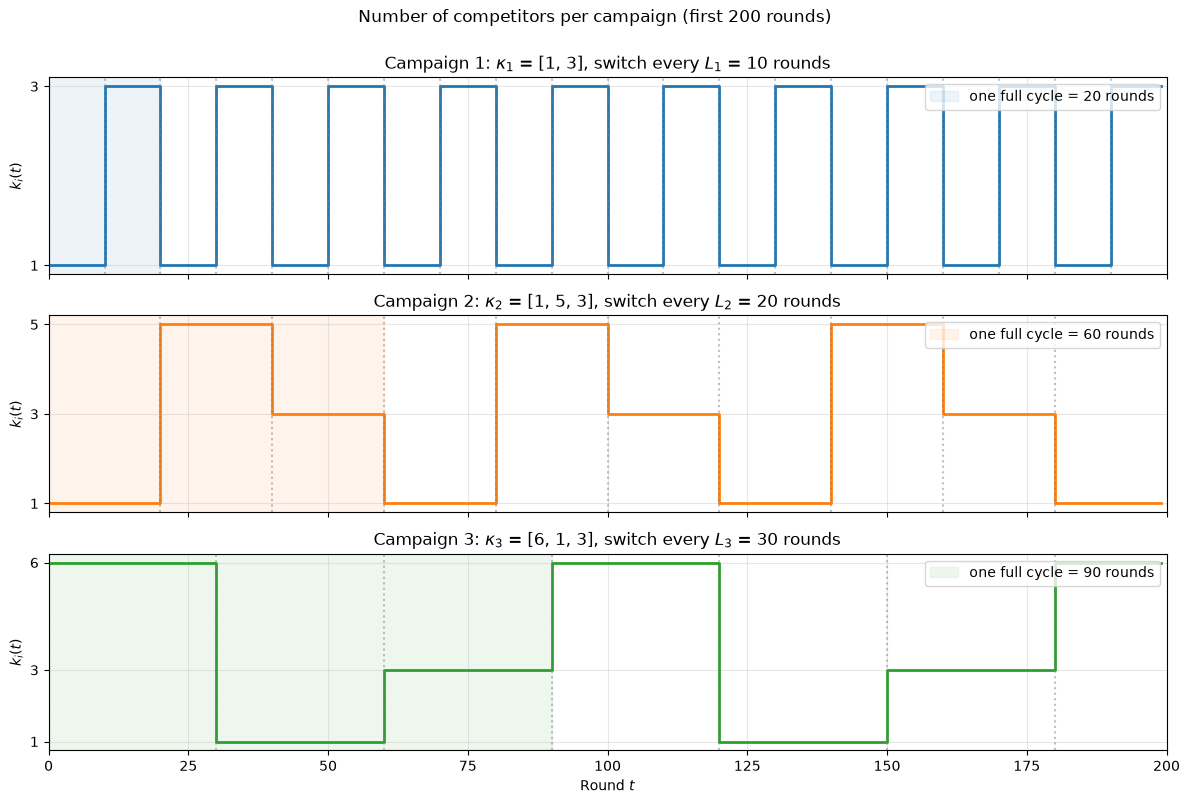
\includegraphics[width=\linewidth,height=0.52\textheight,keepaspectratio]{r3_k_schedule.png}\\[0.05cm]
    {\tiny $k_i(t)$: regimes switch every $L_i$ rounds (first 200 rounds).}
  \end{column}
\end{columns}
\end{frame}

\begin{frame}{R3 --- Baseline: best strategy in hindsight}
\scriptsize
\begin{columns}[T]
  \begin{column}{0.51\textwidth}
    Non-stochastic $\Rightarrow$ benchmark: best \emph{fixed} super-arm distribution
    on the realised sequence, under budget and conflict graph:
    $\OPT=\max_{\gamma\in\Delta_{\mathcal A}}\sum_{t=1}^{T} f_t(\gamma)$
    subject to $\sum_{t=1}^{T} c_t(\gamma)\le B,$
    where $f_t(\gamma)=\sum_{a}\gamma(a)f_t(a)$,
    $c_t(\gamma)=\sum_{a}\gamma(a)c_t(a)$, and
    \begin{align*}
      f_t(a)&=\sum_{i\in S}(v_i-b_i)\,\mathbf 1\{b_i\ge m_i(t)\},\\
      c_t(a)&=\sum_{i\in S} b_i\,\mathbf 1\{b_i\ge m_i(t)\}.
    \end{align*}
    \begin{tabular}{@{}p{0.29\textwidth}l@{}}
      \toprule
      Chosen super-arm & $\OPT$/round\\
      \midrule
      Stationary: $\{1,2\}$, $b{=}(0.4,0.5)$ w.p.\ 1 & $0.061$\\
      Non-stationary: $\{1,3\}$, $b_3\in\{0.4,0.5\}$ & $0.114$\\
      \bottomrule
    \end{tabular}
    \quad Regret $R_T=\OPT-\sum_t f_t(a_t)$.
  \end{column}
  \begin{column}{0.46\textwidth}
    \centering
    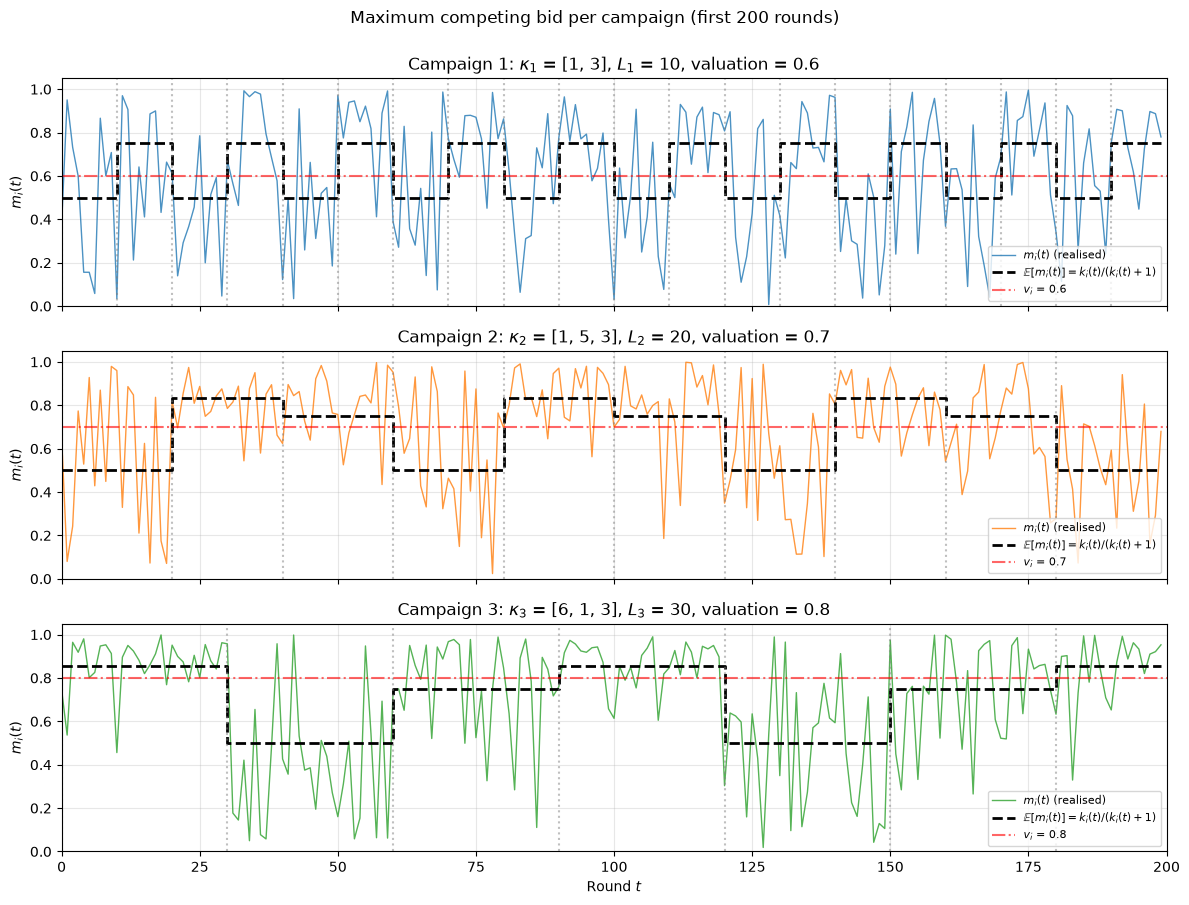
\includegraphics[width=\linewidth,height=0.56\textheight,keepaspectratio]{r3_m_nonstat.png}\\[0.05cm]
    {\tiny Realised $m_i(t)$ with regime mean and valuation $v_i$.}
  \end{column}
\end{columns}
\end{frame}

% - - - - - - - - - - - - - - - - - - - -
\begin{frame}{R3 --- Algorithm: primal-dual pacing over super-arms}
\scriptsize
\textbf{Idea.} An action is a super-arm $a=(S,b)$. Full feedback gives
$f_t(a),\,c_t(a)$ for \emph{every} super-arm, so the primal is an expert problem:
Hedge maximises $L_t(a,\lambda)=f_t(a)-\lambda(c_t(a)-\rho)$ while OGD learns
$\lambda\in[0,1/\rho]$; stop bidding once $B<1$.

\begin{algobox}
\begin{algorithm}[H]
  \scriptsize
  \caption{\scriptsize Primal-dual bidding (full feedback)}
  \KwIn{$B$, $T$, super-arms $\mathcal A$, rates $\eta_p,\eta_d$}
  $\rho\leftarrow B/T$;\; $\lambda_1\leftarrow0$;\; $w_1(a)\leftarrow1$ for all $a$\;
  \For{$t=1,\dots,T$}{
    sample $a_t\sim\gamma_t\propto w_t$; bid $b_t$ on $S_t$; observe wins and $m(t)$\;
    collect $f_t(a_t)$, pay $c_t(a_t)$; $B\leftarrow B-c_t(a_t)$\;
    compute $f_t(a),\,c_t(a)$ for all $a$ from $m(t)$\;
    $w_{t+1}(a)\leftarrow w_t(a)\exp\!\left(\eta_p\,[\,f_t(a)-\lambda_t(c_t(a)-\rho)\,]\right)$\;
    $\lambda_{t+1}\leftarrow\Pi_{[0,\,1/\rho]}\!\left(\lambda_t-\eta_d(\rho-c_t(a_t))\right)$\;
    \If{$B<1$}{play $(\emptyset,\emptyset)$ for the remaining rounds\;}
  }
\end{algorithm}
\end{algobox}
\end{frame}

% - - - - - - - - - - - - - - - - - - - -
\begin{frame}{R3 --- Why it works in both worlds}
\footnotesize
\begin{columns}[T]
  \begin{column}{0.52\textwidth}
    \begin{itemize}
      \item \textbf{No stale averages:} Hedge re-evaluates every super-arm each round from
            the current $m(t)$; $\lambda_t$ prices the budget and makes the primal
            shift to cheaper actions when spending exceeds $\rho$.
      \item \textbf{Same agent, same hyper-parameters} on the stochastic (R2) and the
            highly non-stationary sequence:
            $\eta_p$ on rescaled $L_t$ $=20$, $\eta_d=0.05$, $\lambda_1=0$.
      \item The analysis never uses how $m(t)$ is generated $\Rightarrow$
            sublinear regret in \emph{both} environments:
            $R_{2000}\approx 6$ (stationary) and $\approx 11$ (non-stationary).
      \item \textbf{Guarantee:} regret $O(\sqrt T)$ against the hindsight $\OPT$ and
            $O(\sqrt T)$ budget violation (made exact by the stopping rule).
    \end{itemize}
    \vspace{0.2cm}
    Best of both worlds: stochastic guarantees of UCB-type methods
    \emph{and} adversarial robustness of no-regret learners, with one algorithm.
  \end{column}
  \begin{column}{0.45\textwidth}
    \centering
    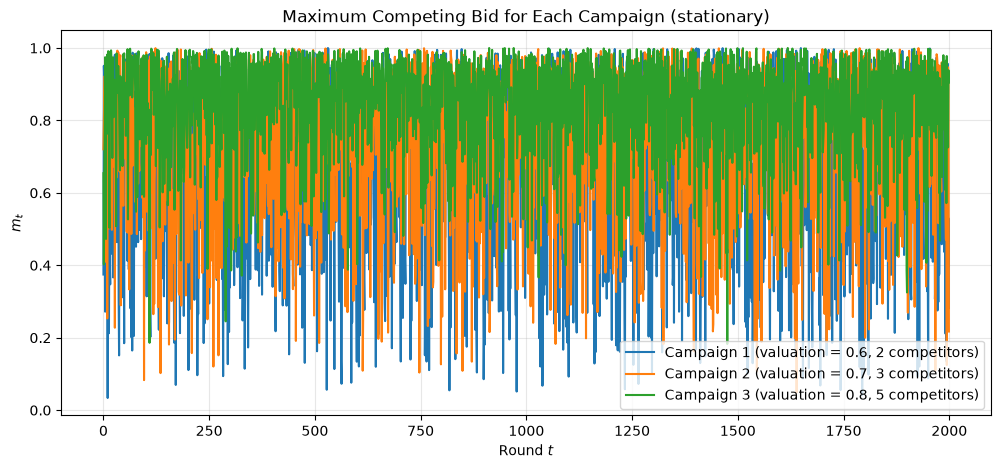
\includegraphics[width=\linewidth,height=0.48\textheight,keepaspectratio]{r3_env_stationary.png}\\[0.1cm]
    {\tiny Stationary sequence (R2 environment): $m_i(t)\sim\mathrm{Beta}(k_i,1)$, $k=(2,3,5)$.}
  \end{column}
\end{columns}
\end{frame}

\begin{frame}{R3 --- Results}
\footnotesize
\centering
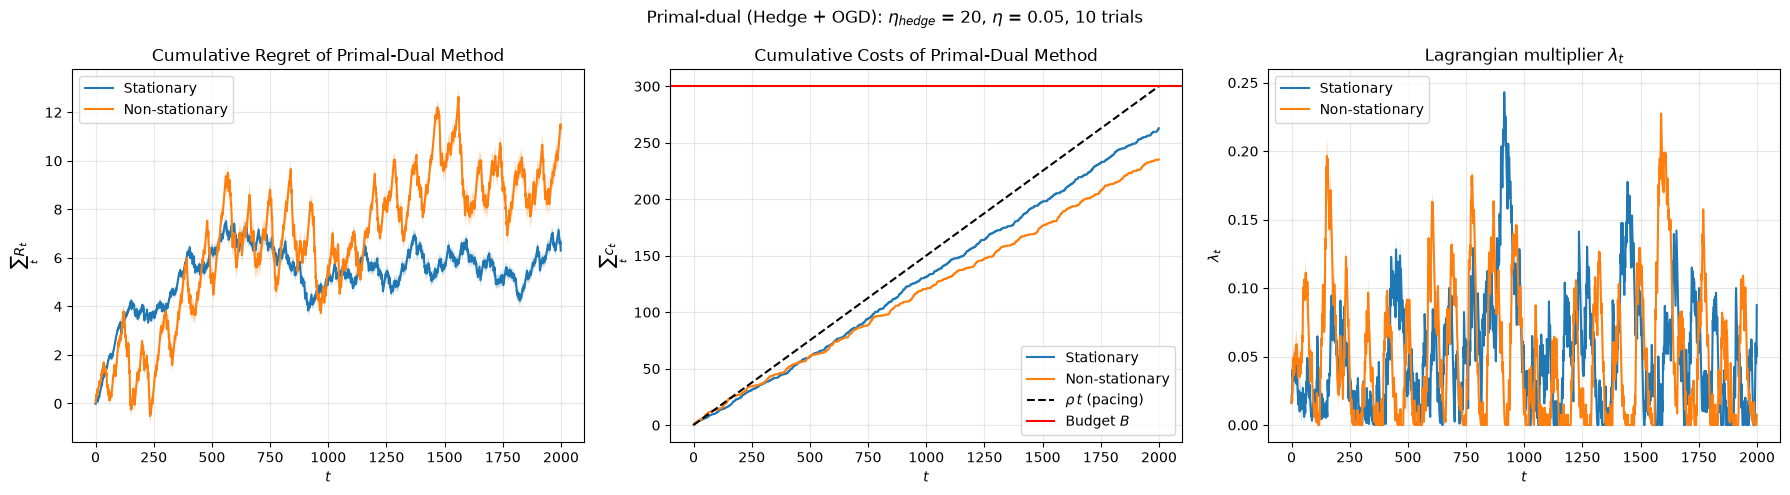
\includegraphics[width=0.94\textwidth,height=0.55\textheight,keepaspectratio]{r3_results.png}\\[0.12cm]
\begin{columns}[T]
  \begin{column}{0.5\textwidth}
    \centering
    \textbf{Stationary:}\\
    regret $6.3\pm0.8$ \quad ($T\cdot\OPT = 121.8$)\\
    spent $262.8/300$
  \end{column}
  \begin{column}{0.5\textwidth}
    \centering
    \textbf{Non-stationary:}\\
    regret $11.3\pm1.5$ \quad ($T\cdot\OPT = 228.7$)\\
    spent $235.2/300$
  \end{column}
\end{columns}
\end{frame}

\begin{frame}{R3 --- Results: learned policy vs clairvoyant}
\footnotesize
\centering
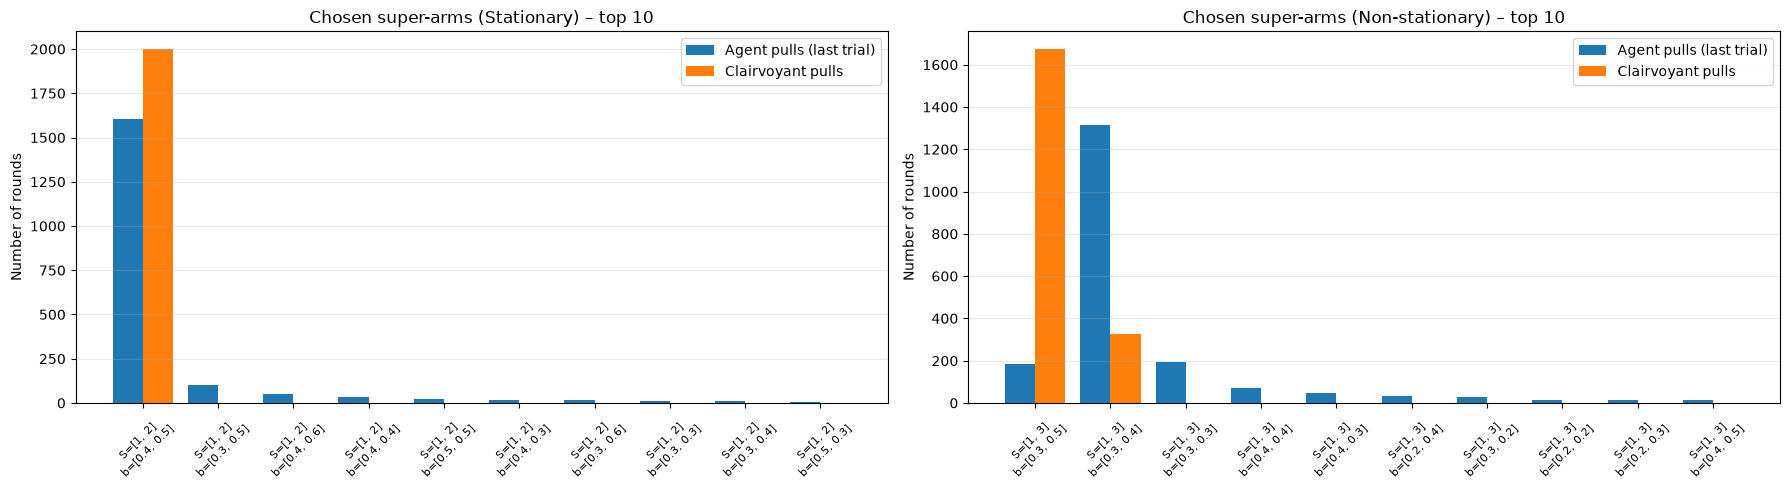
\includegraphics[width=0.94\textwidth,height=0.55\textheight,keepaspectratio]{r3_superarms.png}\\[0.12cm]
\begin{itemize}
  \item \textbf{Stationary:} the agent converges to the clairvoyant super-arm
        ($S=\{1,2\}$, $b=(0.4,0.5)$) in $\sim\!1600$ of $2000$ rounds.
  \item \textbf{Non-stationary:} clairvoyant mixes $b_3\in\{0.4,0.5\}$ on $S=\{1,3\}$;
        agent favours the slightly cheaper $(0.3,0.4)$ --- expected, since $\lambda_t>0$
        penalises cost.
\end{itemize}
\end{frame}
% ####################################################################
\section{Requirement 4 --- Non-stationary environment}
% ####################################################################


\begin{frame}{R4 --- Environment setting}

N

\begin{itemize}
    \item 
\end{itemize}

\end{frame}

% - - - - - - - - - - - - - - - - - - - -
\begin{frame}{R4 --- Algorithm: }

  \begin{algobox}
  \begin{algorithm}[H]
    \scriptsize
    \caption{\scriptsize Combinatorial UCB with Sliding Window}
    \KwIn{... window size ${W}$ ...}
    \For{$t = 1,\dots,T$}{
        % On \texttt{update()}:\;
        % \KwIn{played arms, reward, cost}\;
        % Record "empty" entry for non-played arms\;
        % \If{$t \gt W$}{
        %     \If{$history(t-W) not empty$}{
        %         
        %     }
        % }
      \ForEach{$b \in \bidset$}{
        $\overline{f}_t(b)\leftarrow\frac{1}{N_{W, t-1}(b)}\Sigma_{t'=max(1, t-W)}^{t'=t}f_{t'}(b)\mathbb{I}(b_{t'}=b)$\;
        $\overline{f}_t^{UCB}(b)\leftarrow\overline{f}_t(b)+\sqrt{\frac{2\log(T)}{N_{W, t-1}(b)}}$\;
        $\overline{c}_t(b)\leftarrow\frac{1}{N_{W, t-1}(b)}\Sigma_{t'=max(1, t-W)}^{t'=t}c_{t'}(b)\mathbb{I}(b_{t'}=b)$\;
        $\overline{c}_t^{UCB}(b)\leftarrow\overline{c}_t(b)-\sqrt{\frac{2\log(T)}{W, N_{t-1}(b)}}$\;
      }
      Compute $\gamma_t$ solution of the LP defining $OPT_{t}$ \;
      
      Bid $b_t \sim \gamma_t$ \;
      Observe $f_t(b_t)$ and $c_t(b_t)$\;
      $B\leftarrow B-c_t(b_t)$\;
      \If{$B<1$} {
        Terminate\;
      }
    }
  \end{algorithm}
  \end{algobox}

\end{frame}

% - - - - - - - - - - - - - - - - - - - -
\begin{frame}{R4 --- Algorithm }

  \begin{algobox}
  \begin{algorithm}[H]
    \scriptsize
    \caption{\scriptsize Combinatorial UCB with Change Detection}
    \KwIn{... change ${\epsilon}$, change detection threshold ${h}$ ...}
    \tau = (1,...) \;
    
    \For{$t = 1,\dots,T$}{
      \ForEach{$b \in \bidset$}{
        $\overline{f}_t(b)\leftarrow\frac{1}{N_{\tau_b, t-1}(b)}\Sigma_{t'=\tau_b}^{t'=t}f_{t'}(b)\mathbb{I}(b_{t'}=b)$\;
        $\overline{f}_t^{UCB}(b)\leftarrow\overline{f}_t(b)+\sqrt{\frac{2\log(T)}{N_{\tau_b, t-1}(b)}}$\;
        $\overline{c}_t(b)\leftarrow\frac{1}{N_{\tau_b, t-1}(b)}\Sigma_{\tau_b}^{t'=t}c_{t'}(b)\mathbb{I}(b_{t'}=b)$\;
        $\overline{c}_t^{UCB}(b)\leftarrow\overline{c}_t(b)-\sqrt{\frac{2\log(T)}{\tau_b, N_{t-1}(b)}}$\;
      }

     Same as other Combinatorial UCB... \;

     \If{\texttt{change-detected}($f_t(b_t), c_t(b_t)$)}{
        $\tau_b \leftarrow t$ \;
     }
      
      $B\leftarrow B-c_t(b_t)$ ...\;
    }
  \end{algorithm}
  \end{algobox}


\end{frame}

\begin{frame}{R4 --- Results}

\end{frame}

% ####################################################################
\section{Discussion \& Conclusion}
% ####################################################################

\begin{frame}{Discussion}

\end{frame}

\begin{frame}{Conclusions}
 
\end{frame}

\begin{frame}[plain,c]
  \centering
  {\Huge Thank you!}
\end{frame}


% ####################################################################
\appendix
% ####################################################################



\end{document}
